\documentclass{sigchi}

\usepackage[utf8]{inputenc}

% Arabic page numbers for submission.  Remove this line to eliminate
% page numbers for the camera ready copy
% \pagenumbering{arabic}

% Load basic packages
\usepackage{balance}       % to better equalize the last page
\usepackage{blindtext}
\usepackage{graphics}      % for EPS, load graphicx instead 
\usepackage[T1]{fontenc}   % for umlauts and other diaeresis
\usepackage{txfonts}
\usepackage{mathptmx}
\usepackage[pdflang={en-US},pdftex]{hyperref}
\usepackage{color}
\usepackage{booktabs}
\usepackage{textcomp}
\usepackage{tikz}

% Some optional stuff you might like/need.
\usepackage{microtype}        % Improved Tracking and Kerning
% \usepackage[all]{hypcap}    % Fixes bug in hyperref caption linking
\usepackage{ccicons}          % Cite your images correctly!
% \usepackage[utf8]{inputenc} % for a UTF8 editor only

% If you want to use todo notes, marginpars etc. during creation of
% your draft document, you have to enable the "chi_draft" option for
% the document class. To do this, change the very first line to:
% "\documentclass[chi_draft]{sigchi}". You can then place todo notes
% by using the "\todo{...}"  command. Make sure to disable the draft
% option again before submitting your final document.
\usepackage{todonotes}

% Paper metadata (use plain text, for PDF inclusion and later
% re-using, if desired).  Use \emtpyauthor when submitting for review
% so you remain anonymous.
\def\plaintitle{Influência da Mídia no Mercado de Ações}
\def\plainauthor{}
\def\emptyauthor{}
\def\plainkeywords{Classificação, Perfil.}
\def\plaingeneralterms{Documentation, Standardization}

% llt: Define a global style for URLs, rather that the default one
\makeatletter
\def\url@leostyle{%
  \@ifundefined{selectfont}{
    \def\UrlFont{\sf}
  }{
    \def\UrlFont{\small\bf\ttfamily}
  }}
\makeatother
\urlstyle{leo}

% To make various LaTeX processors do the right thing with page size.
\def\pprw{8.5in}
\def\pprh{11in}
\special{papersize=\pprw,\pprh}
\setlength{\paperwidth}{\pprw}
\setlength{\paperheight}{\pprh}
\setlength{\pdfpagewidth}{\pprw}
\setlength{\pdfpageheight}{\pprh}

% Make sure hyperref comes last of your loaded packages, to give it a
% fighting chance of not being over-written, since its job is to
% redefine many LaTeX commands.
\definecolor{linkColor}{RGB}{6,125,233}
\hypersetup{%
  pdftitle={\plaintitle},
% Use \plainauthor for final version.
%  pdfauthor={\plainauthor},
  pdfauthor={\emptyauthor},
  pdfkeywords={\plainkeywords},
  pdfdisplaydoctitle=true, % For Accessibility
  bookmarksnumbered,
  pdfstartview={FitH},
  colorlinks,
  citecolor=black,
  filecolor=black,
  linkcolor=black,
  urlcolor=linkColor,
  breaklinks=true,
  hypertexnames=false
}

% create a shortcut to typeset table headings
% \newcommand\tabhead[1]{\small\textbf{#1}}

% End of preamble. Here it comes the document.
\begin{document}

\title{\plaintitle}

\numberofauthors{3}
\author{%
  \alignauthor{Higor Oliveira\\
    \affaddr{Universidade Federal de Mato Grosso do Sul}\\
    \affaddr{Coxim, Brasil}\\
    \email{higor.oliveira@aluno.ufms.br}}\\
  \alignauthor{Rafael Viana\\
    \affaddr{Universidade Federal de Mato Grosso do Sul}\\
    \affaddr{Coxim, Brasil}\\
    \email{rafael.viana@aluno.ufms.br}}\\
 \alignauthor{Ramon Santos\\
	\affaddr{Universidade Federal de Mato Grosso do Sul}\\
	\affaddr{Coxim, Brasil}\\
	\email{ramon.santos@aluno.ufms.br}}\\	
}

\maketitle

\begin{abstract}

Este trabalho tem como iniciativa mostrar como polêmicas propagadas pela mídia podem influenciar no mercado de ações da bolsa de valores, através de notícias referentes principalmente ao meio político e socioeconômico\end{abstract}
.

\keywords{Bolsa de valores, análise de sentimento social, política, mídia.}

\section{Introdução}
A mídia é popularmente conhecida por sua força e poder de influência para o lado negativo. Isso fica mais nítido quando por meio de toda essa influência, ela passa a induzir nas pessoas uma ideia ou mesmo um ponto de vista já formado sobre determinado assunto. 

Por outro lado, se bem utilizada, ela pode contribuir de diversas formas, no mercado da bolsa de valores, por exemplo, pode ajudar os investidores a investir em suas ações no momento certo.

Neste trabalho foi realizada uma pesquisa de como a mídia tem influência direta na bolsa de valores, mais especificamente nas ações de bancos, para isso foram utilizados como exemplo dois dos cinco maiores bancos nacionais, sendo eles: Banco do Brasil e Bradesco.

 Baseado nos dados recolhidos no estudo, foi concluído que: 
 \begin{itemize}
 
 \item{Este se trata de um problema de classificação;}
 \item{Existe uma relação entre polêmicas no meio politico e a queda de ações dos bancos.}
 
 \end{itemize}
Com isso foi criada a seguinte hipótese: 

\textit{
Quando algum escândalo ou polêmica de grandes proporções é noticiado pela mídia, os investidores tendem a tirar o dinheiro investido na bolsa de valores pelo receio de suas ações desvalorizarem.
}

\subsection{Objetivo}

\begin{itemize}
	
	\item Calcular atraves de algumas variaveis quando uma suposta queda e o momento ideal para investir em ações bancarias.
	\item 
\end{itemize}


\section{Metodologia}
Foram inseridas as ações BBAS3 (Banco do Brasil) e BBDC4 (Bradesco) na ferramenta de visualização de gráficos presente no site www.br.advfn.com, que gerou o seguinte gráfico: aeuhfuane 

 \begin{figure}[!htb]
\centering
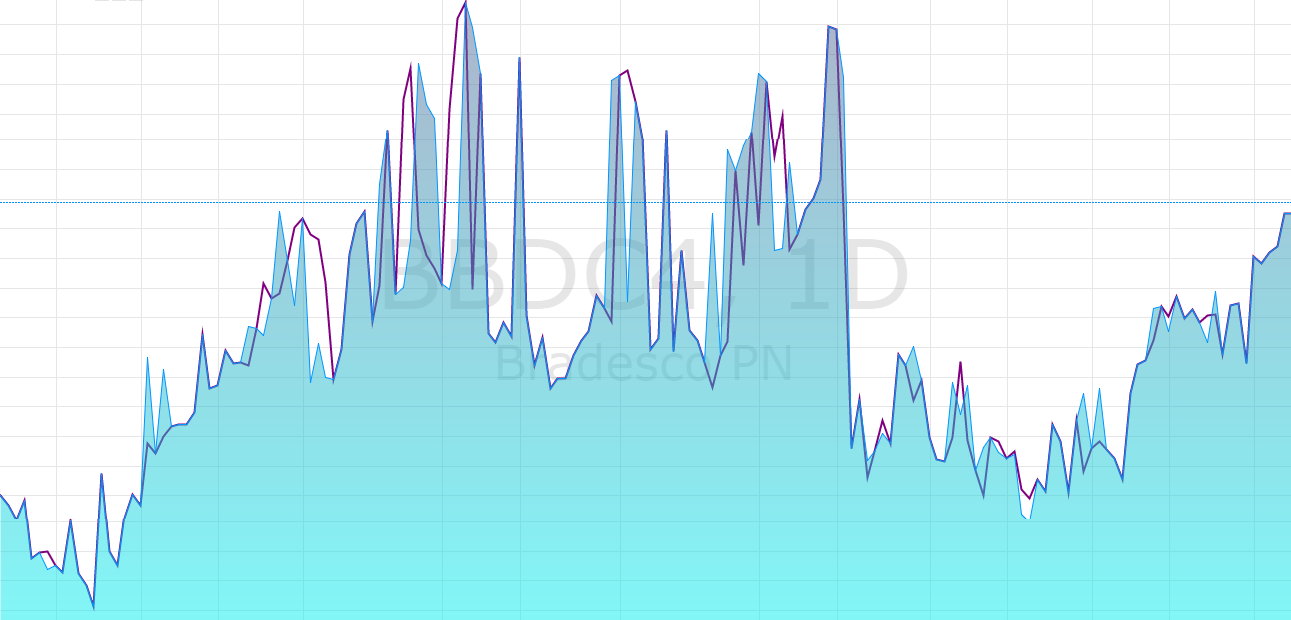
\includegraphics[scale=0.27]{./figures/figura1.png}
\caption{Gráfico de ações BBAS3 e BBDC4}
\label{fig1}
\end{figure}

É possível notar visualmente, que as linhas geradas são muito semelhantes. Foi notado então um ponto onde a queda é notável para ambos os bancos. Figura \ref{fig2}


 \begin{figure}[!htb]
	\centering
	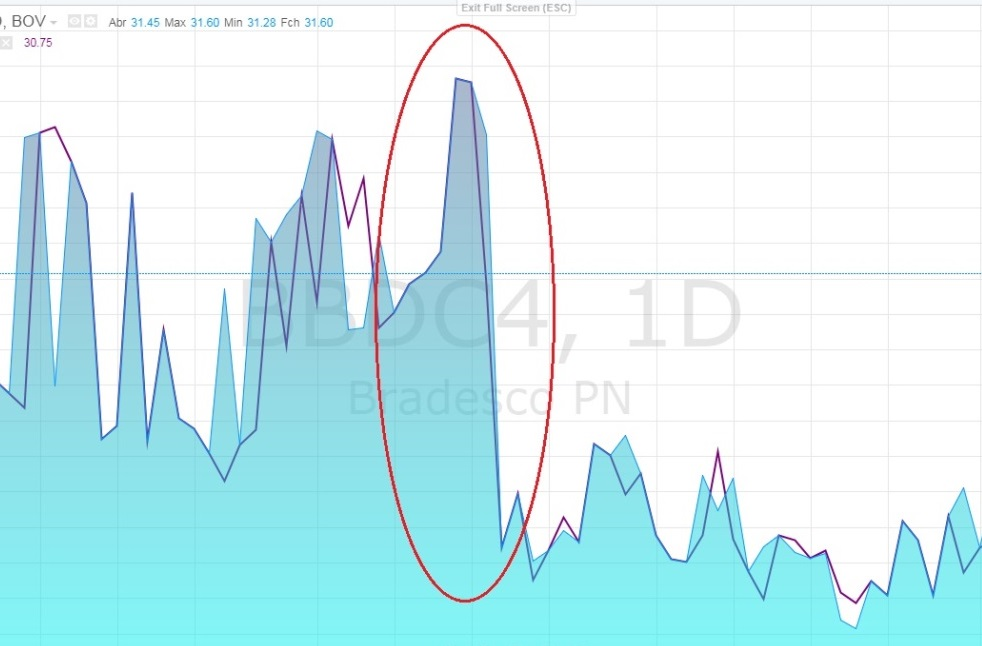
\includegraphics[scale=0.8]{./figures/figura5.jpg}
	\caption{Queda nas ações bancarias BBAS3 e BBDC4 }
	\label{fig2}
\end{figure}

Analisando mais a fundo, a queda ocorreu literalmente do dia para a noite. Na tarde de 17/05/2017 as ações ainda estavam em alta, na manhã do dia seguinte (18/05/2017) sofreram uma perda enorme. Partindo deste ponto, realizamos uma busca em sites de notícias no âmbito de encontrar algo que estivesse relacionado ao tema e que tivesse o poder de afetar o mercado bancário. Dentre as encontradas, a notícia que possivelmente afetou o mercado é a seguinte.

\begin{figure}[!htb]
	\centering
	
\includegraphics[scale=0.4]{./figures/figura3.jpg}
	\caption{Delação JBS.}
	\label{figRotu}
\end{figure}

Para provar que não se trata de uma simples coincidência, foi realizada uma procura no gráfico, buscando por outro declínio, utilizando as mesmas características visuais da 1ª queda. Foi detectada então, em Novembro de 2016, uma muito semelhante.

\begin{figure}[!htb]
\centering
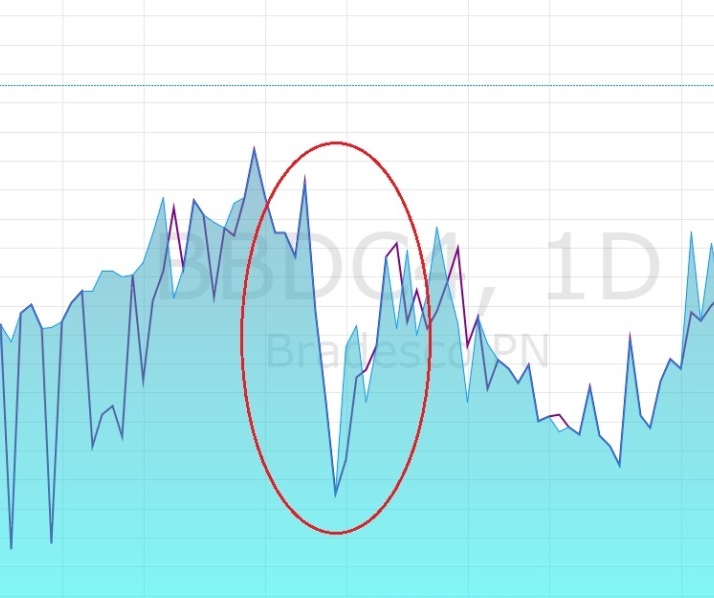
\includegraphics[scale=0.85]{./figures/queda-2016.jpg}
\caption{Donald Trump é eleito.}
\label{figRotu}
\end{figure}
Diferentemente da queda de Maio/2017, a queda de Novembro/2016 foi mais espaçada, ocorreu aproximadamente do dia 08 ao dia 11 de Novembro.

\begin{figure}[!htb]
	\centering
	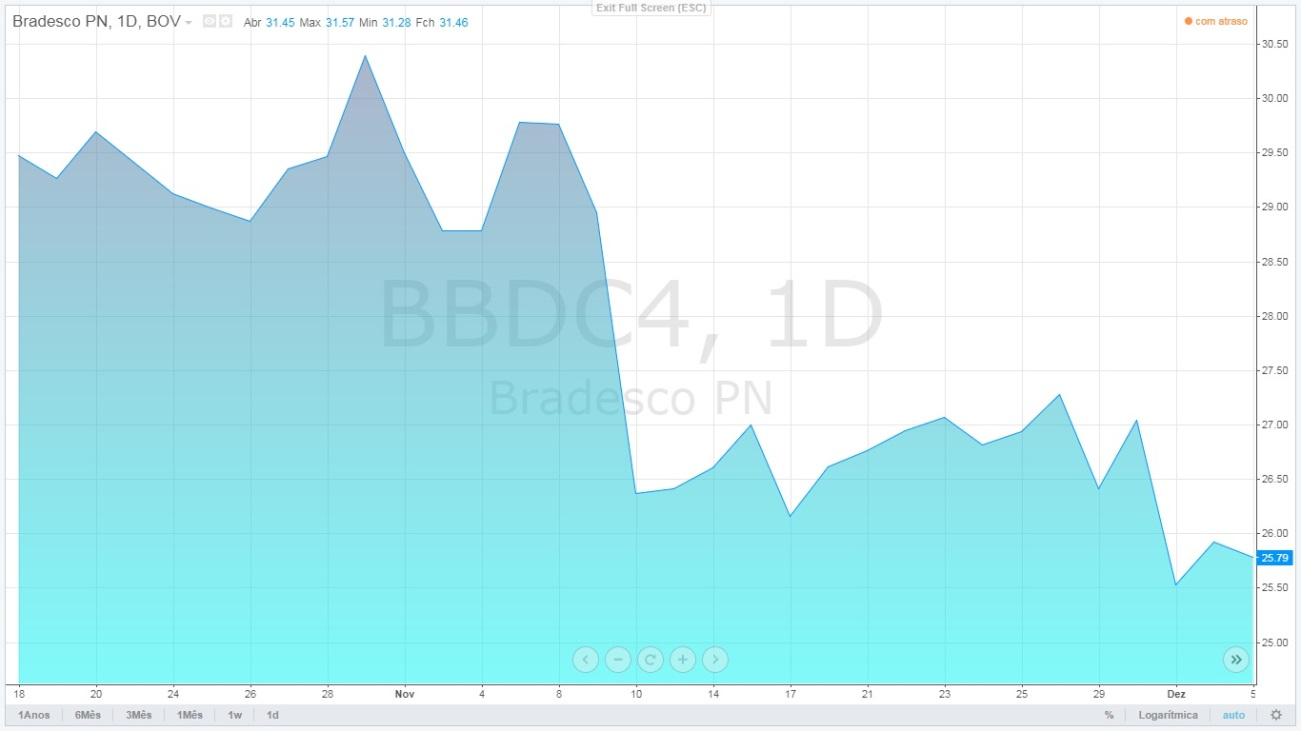
\includegraphics[scale=0.5]{./figures/figura6.jpg}
	\caption{Legenda}
	\label{figRotu}
\end{figure}
Então foi feita a mesma busca por notícias realizada anteriormente, que retornou o seguinte resultado: 
\begin{figure}[!htb]
	\centering
	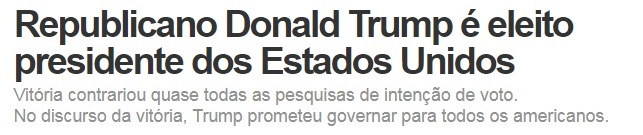
\includegraphics[scale=0.4]{./figures/figura7.jpg}
\caption{Donald Trump é eleito.}
	\label{figRotu}
\end{figure}

Com esse resultado em mãos, foi compreendido que prever quando ocorrerá uma queda na bolsa é extremamente difícil, se não impossível, e por este motivo, não deve ser um objetivo a ser atingido. O objetivo correto então é tentar calcular o “tamanho da queda” que já está em andamento, para saber se este é um bom momento para investir. Este cálculo poderia envolver, por exemplo:
\begin{enumerate}
\item A quantidade dos veículos de comunicação que foram utilizados para propagar a notícia. (Televisão, rádio, jornais, etc.).

\item A quantidade de pessoas que tem acesso a essa informação.
Como está a “popularidade” desta notícia nas redes sociais (Facebook, Twitter entre outras).
\end{enumerate}


Com isso, as notícias poderiam ser classificadas em: 
\begin{enumerate}
	\item Pouca probabilidade de queda;
	
	\item Média probabilidade de queda;
	Como está a “popularidade” desta notícia nas redes sociais (Facebook, Twitter entre outras).
	\item Alta probabilidade de queda.
\end{enumerate}



Assim, com os cálculos corretos e com base nessa classificação, os acionistas teriam um “termômetro” com base no atual momento da sociedade, indicando se é ou não um momento apropriado para investir.

\section{Conclusão}

A conclusão obtida com este estudo é de que existe uma relação entre grandes notícias no meio político/econômico e as quedas nas ações bancárias na bolsa de valores. Isto se dá pelo conceito do comportamento de manada: por medo de uma polêmica desvalorizar suas ações, alguns acionistas tendem a retirar o que foi investido, o que faz toda a “manada” seguirem seus passos. Essa relação pode ser calculada, não para prever futuras quedas, e sim para saber em qual queda valeria mais a pena investir.


% BALANCE COLUMNS
\balance{}

% REFERENCES FORMAT
% References must be the same font size as other body text.
\bibliographystyle{SIGCHI-Reference-Format}
\bibliography{sample}

\end{document}

%%% Local Variables:
%%% mode: latex
%%% TeX-master: t
%%% End:
